\documentclass[11pt]{article}
\usepackage{a4wide}
\usepackage{float}
\usepackage{graphicx}
\usepackage{hyperref}

\begin{document}

\begin{titlepage}
\title{Openseekmap}
\author{Thor Dossche}
\date{Academiejaar 2020 - 2021}
\maketitle
\thispagestyle{empty}
\end{titlepage}


\section{Inleiding}
Het programma openseekmap zal voor een gegeven query de 5 best matchende plaatsnamen uit een meegegeven databank terug geven. We bereiken dit door het inlezen van de databank in het geheugen, waarna de query $z$ opgesplitst wordt op spaties: $ z = z_1 \ldots z_n $. \\
Bij het zoeken houden we een array $matches$ van gelinkte lijsten bij. We zoeken nu voor ieder stuk $z_i$ uit een opsplitsing van $z$ apart naar matches en voegen deze toe aan $matches[i]$. Na het zoeken van een opsplitsing zullen we alle resultaten uit $matches$ recursief met elkaar mergen en toevoegen aan een ranking. Dit proces herhalen we voor alle mogelijke combinaties van opsplitsingen van $z$. De ranking zal iedere totale match een score geven en enkel de 5 matches met de hoogste score bijhouden.\\ 
\\
Bij het zoeken van een stuk $z_i$ maken we een selectie van matches met een editeerafstand kleiner of gelijk aan $\min(3,1+|z_i|)$. Met een $shift\_and$ algoritme maken we een preselectie of het wel de moeite loont om de editeerafstand te berekenen. De $shift\_and$ heeft een $budget$ van 6. Dit aangezien enkel insertion, deletion, replacement geïmplementeed zijn maar ook het wisselen van 2 letters een mogelijkheid is. Stel in het geval van 3 wissels op verschillende plaatsen is dit hetzelfde als 3 insertions en 3 deletions (of andere combinaties) waardoor we aan een budget van 6 komen. Als $shift\_and$ teruggeeft dat $z_i$ op afstand ten hoogste 6 van de huidige entry ligt, berekenen we hiervan de editeerafstand. Stel dat de lengte van de huidige entry kleiner is dan die van $z_i$ zullen we altijd de editeerafstand berekenen.

\section{Onderzoek}
Alle onderzoeksopdrachten zijn gedaan voor 2.4 UTF-8, de resultaten in de tabellen zijn dus resultaten door met ascii te werken.

\subsection{Algoritmes voor editeerafstand}

Voor de editeeraftand ben ik begonnen met een algoritme die een volledige matrix bijhoudt. Op deze matrix voeren we rij per rij het editeerafstand algoritme uit. Aangezien dit meer ruimte inneemt dan nodig heb ik daarna het algoritme aangepast zodat er maar 3 rijen meer gebruikt worden en iedere iteratie wisselen de pointers van de rijen. De 3 gebruikte rijen zijn $next$, $prev$ en $swap$. De $next$ array bevat de resultaten van de editeerafstanden die in de huidige iteratie worden berekend. $prev$ bevat die van de vorige iteratie en $swap$ die van 2 iteraties geleden. De $swap$ is nodig om het wisselen van 2 opeenvolgende letters mogelijk te maken. Aan het einde van iedere iteratie wisselen de pointers als volgt: $ next -> prev -> swap -> next $ dus de oude $swap$ zal gebruikt worden om de resultaten van de volgende iteratie in weg te schrijven. \\
\\
\newpage
In onderstaande tabel zijn de resultaten te vinden die het verschil aantonen om editeerafstanden te berekenen met de matrix t.o.v. de pointer implementatie. Het is duidelijk dat het gebruik van de pointer implementatie in de praktijk zeker de voorkeur geniet.
\\
\begin{table}[H]
        \centering
        \begin{tabular}{ |c|c|c|c| }
                \hline
                query & matrix & pointers & speedup (\%)\\
                \hline
                a                              & 0.007245 & 0.007248 & -0.04\\
                gent                           & 0.00925 & 0.00892 & 3.70\\
                de sterre gent                 & 0.01604 & 0.01429 & 12.25\\
                station gent-sint-pieters gent & 0.02634 & 0.02171 & 21.33\\
                \hline
        \end{tabular}
        \caption{Tijd in s om 10000 editeerafstanden te berekenen}
\end{table}

Tijdens het zoeken zal er eerst een preselectie gemaakt worden door een shift\_and algoritme, maar meer hierover in 2.3 Bounding.\\
\\

\subsection{Preprocessing}
Als preprocessing stap heb ik 3 dingen geprobeerd. Om te beginnen heb ik de database in een gelinkte lijst ingelezen. Later heb ik de databank in een datamap ingelezen. Deze datamap is een lijst van gelinkte lijsten waarbij een entry met lengte $n$ in de gelinkte lijst op positie $n-1$ van de datamap zal worden toegevoegd. De laatste stap was de databank in een datamap inlezen en deze datamap dan te herschrijven in het geheugen. De tijden om dit te doen staan in onderstaande tabel.
\begin{table}[H]
        \centering
        \begin{tabular}{ |c|c|c|c|c| }
                \hline
                dataset & \#entries & linkedlist & datamap & datamap + rewrite\\
                \hline
                belgie  & 169983 & 0.15 & 0.10 & 0.21\\
                benelux & 485829 & 0.41 & 0.28 & 0.57\\
                \hline
        \end{tabular}
        \caption{Tijd in s om een database in te lezen}
\end{table}

De reden waarom we de datamap willen herschrijven, is op het eerste zicht niet onmiddellijk duidelijk. Dit heeft namelijk te maken met het proberen optimaal gebruiken van caching. Bij het inlezen van de databank staan de strings van verschillende grootte door elkaar. \\Hierdoor zullen de entries van dezelfde lengte niet perse naast elkaar zitten in het geheugen. Tijdens het zoeken zal er steeds lijst per lijst worden gezocht en dus de entries met dezelfde lengte zullen na elkaar opgevraagd worden aan het geheugen. Om de caches beter te gebruiken willen we dus dat de entries met dezelfde lengte naast elkaar zitten in het geheugen. Dit is de reden voor het herschrijven van de datamap.\\
\\
Waarom we de database in deze datamap inlezen wordt hieronder bij Bounding besproken.
\newpage
\subsection{Bounding}

We hebben nu onze database in een datamap ingelezen. Aangezien we enkel entries op een editeeraftand $\min(3,1+|z_i|)$ bekijken als mogelijke match moeten we dus maar een deel van de databank overlopen, namelijk entries met lengte $x \in [n-2, n+2]$ met $n$ de lengte van $z_i$. Deze komen overeen met ten hoogste 2 verwijder- of toevoegoperaties. Andere entries zullen sowieso een grotere dan de maximaal toegestane editeeraftand hebben. Met de gebruikte datamap is dit efficiënt te doen en kunnen we onmiddellijk deze entries overlopen. De zoektijden van enkele queries staan in onderstaande tabel.\\
\begin{table}[H]
        \centering
        \begin{tabular}{ |c|c|c|c|c|c| }
                \hline
                query & linkedlist & datamap & datamap + rewrite & speedup (\%)\\
                \hline
                steyneveld                 & 0.035 & 0.024 & 0.017 & 105.9\\
                de sterre gent             & 0.238 & 0.129 & 0.084 & 183.3\\
                kollegelaan kortrijk       & 0.198 & 0.074 & 0.057 & 247.4\\ 
                hoge bosstraat eeklo       & 0.768 & 0.552 & 0.485 & 58.4\\
                ottignies-louvain-la-neuve & 0.190 & 0.0075 & 0.0067 & 2735.8\\

                \hline
        \end{tabular}
        \caption{Tijd in s om een query te zoeken zonder databank inlezen}
        \label{searchtime}
\end{table}

We zien dat het een pak efficiënter is om met een datamap i.p.v. een gelinkte lijst te werken. Het is ook nog net wat voordeliger om met een herschreven datamap te werken dan de rechtstreeks ingelezen datamap. De vraag is nu vanaf hoeveel queries is de kost van het herschrijven van de datamap te rechtvaardigen? Onderstaande grafiek toont de gemiddelde zoektijd van 50 simulaties. Deze simulaties laden de databank in en zullen dan $0,...,20$ willekeurige queries zoeken. We zien dat het al vrij snel voordelig is om met een herschreven datamap te werken. Hoe meer queries we zoeken hoe voordeliger.

\begin{figure}[H]
        \centering
        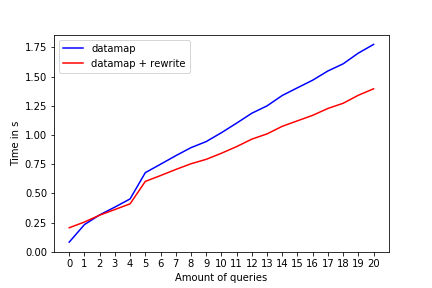
\includegraphics[scale=0.75]{datamap_vs_rewrite.png}
        \caption{Zoeken met een datamap en een herschreven datamap}
\end{figure}

\newpage

Een volgende optimalisatie is dat voor we de editeeraftand van een entry berekenen we een $shift\_and$ algoritme zullen gebruiken, om te kijken of we de editeeraftand wel moeten berekenen. Het geïmplementeerde $shift\_and$ algoritme heeft enkele beperkingen en zal ook niet altijd gebruikt worden, maar dat werd in de inleiding al aangehaald. Ondanks zijn beperkingen kunnen we in onderstaande tabel zien dat het gebruik er van, om een preselectie maken, toch een mooie snelheidswinst oplevert.

\begin{table}[H]
        \centering
        \begin{tabular}{ |c|c|c|c|c| }
                \hline
                query & without shift\_and & with shift\_and & speedup (\%)\\
                \hline
                steyneveld                 & 0.136 & 0.080 &  70.0\\
                de sterre gent             & 0.216 & 0.135 &  60.0\\
                kollegelaan kortrijk       & 0.047 & 0.027 &  74.1\\ 
                hoge bosstraat eeklo       & 0.641 & 0.541 &  18.5\\
                ottignies-louvain-la-neuve & 0.014 & 0.007 &  100.0\\

                \hline
        \end{tabular}
        \caption{Tijd in s om een query te zoeken met datamap + rewrite}
\end{table}
\subsection{UTF-8}
We willen niet alle karakteristieke vectoren van de karakters in de UTF-8 karakterset opslaan. Maar aangezien de karakters die we voornamelijk zullen nodig hebben de karakters zijn uit de ascii dataset kunnen we voor deze wel alle vectoren bijhouden. Dit is dan ook de gebruikte aanpak. Hou een array van de karakterestieke vectoren bij en elke keer als er een oproep wordt gedaan, kijken we of het huidige teken $< 128$ is. Indien het geval geven we de bijhorende vector uit de array terug. Anders zullen we over het te matchen woord itereren en zo de karakterestieke vector opstellen voor het gevraagde letterteken.

\section{Complexiteit}

In dit deel gaan we even kijken om een beeld te krijgen van de complexiteit van het volledige zoekalgoritme. Hiervoor zullen we kijken naar het slechtste geval omdat het anders verre van eenvoudig is om een analyse te maken.\\\\
Voor het inlezen van de databank met $x$ entries zullen we dit in $O(x)$ kunnen doen, iedere entry wordt toegevoegd aan de datamap, dit is hetzelfde als toevoegen aan een gelinkte lijst. In de gebruikte implementatie kan dat in 1 keer. Indien we de datamap herschrijven zal de kost $2x$ zijn.\\
\\
We zoeken nu naar een string $z$ met lengte $n$, we kunnen $z$ opsplitsen in $m$ delen. Hier stellen we dat alle $z_i$ dezelfde lengte hebben ($k$) en dat alle database entries een lengte hebben $\in[k-2, k+2]$. Hierdoor hebben we het slechtste geval als $z$ in $m$ delen is opgesplit. Voor iedere $z_i$ zullen alle entries overlopen worden (kost $mx$). We zullen het aantal iteraties per combinatie van opsplitsingen hieraan gelijk stellen. Het aantal combinaties van opsplitsingen die we kunnen maken is $2^{m-1}$. In totaal levert dit een kost van $2^{m-1}*mx$.\\
\\
Voor de hoeveelheid werk die $shift\_and$ en $edit\_distance$ gebruiken, gaan we weer van het slechtste geval uit. Dit is wanneer we $z$ in $m$ stukken splitsen en dat alle entries in de databank lengte $k+2$ hebben. Alle andere gevallen van opsplitsingen zullen minder werk zijn. Omdat alle entries lengte $k+2$ zal voor iedere entry het $shift\_and$ algoritme opgeroepen worden, dus kost van $x$ keer $k+2$. Als we nog eens van het slechtste geval uitgaan, de entry ligt op ten hoogste distance 6, zal voor iedere entry ook het $edit\_distance$ algoritme worden opgroepen. Dit geeft een kost van $x$ keer $k*(k+2)$. Dit samen geeft ons een kost van $x((k+2) + k(k+2))$\\
\\
Een laatste deel van de complexiteit is de hoeveelheid matches die gevonden wordt voor een opsplitsing van $z$. Ook hier gaan we weer van het slechtste geval uit, $z$ is gesplitst in $m$ delen en alle x entries in de database liggen op distance $<= 3$ voor alle delen van de opsplitsing van $z$. Dit wil zeggen dat voor iedere $z_i$ de volledige database gematcht zal worden. Als we nu de matches combineren, zal dit een totaal van $x^m$ combinaties opleveren. Voor al deze combinaties zal een score worden berekend, laten we zeggen dat het werk hiervoor constant is en de complexiteit niet beïnvloedt.\\
\\
Als we alles nu combineren, waarbij we stellen dat iedere opsplitsing even veel werk is als het slechtste geval, krijgen we: \\

$O(2x + 2^{m-1}*(mx*((k+2) + k(k+2)) + x^m))$\\
$  => O(x^m)$\\

De tijd van het algoritme zal dus voornamelijk afhangen van hoeveel matches er voor de opsplitsingen gevonden worden en hoe groot $m$ is. Ook al is het berekenen van de score niet veel werk toch zal dit in slechte gevallen het meeste tijd kosten. Dit valt in de praktijk sterk op. Als we kijken naar Table \ref{searchtime} dan zien we dat de query 'hoge bosstraat eeklo' veel meer tijd nodig heeft dan de anderen. Dit is omdat er zeer veel combinaties gemaakt moeten worden bij de opsplitsing ['hoge', 'bosstraat', 'eeklo'] waardoor het recursief combineren veel tijd kost.\\
\\
Een extra voorbeeld om dit te illustreren:
\begin{table}[H]
        \centering
        \begin{tabular}{ |c|c|c|c|c| }
                \hline
                query & linkedlist & datamap & datamap + rewrite & max combinations for matches\\
                \hline
                rue du des avenue  & 5.77 & 4.17 & 4.02 & 7375824\\
                vieux rue de namur & 0.80 & 0.42 & 0.26 & 111150\\
                \hline
        \end{tabular}
        \caption{Tijd in s om een query te zoeken}
\end{table}
De query "rue du des avenue" is natuurlijk een geknusteld voorbeeld om mijn stelling aan te tonen en is geen werkelijke query. Maar we zien dat er een heel groot verschil is van tijd voor 2 queries met even veel opsplitsingen.
\end{document}
